\section{Brechung}

Fällt ein Lichtstrahl auf die Grenzfläche zweier Medien, so dringt ein Teil des einfallenden Lichtes in das zweite Medium ein. \\
Die auftrentende Richtungsänderung wird als \textbf{Brechung} bezeichnet. \\
Der in das zweite Medium eindringende Strahl wird \textbf{gebrochener Strahl} genannt.


\subsection{Brechungsgesetz / Geschwindigkeit}

\begin{minipage}[t]{0.34\columnwidth}
    \textbf{Achtung:} Es gilt $n_1 < n_2$

    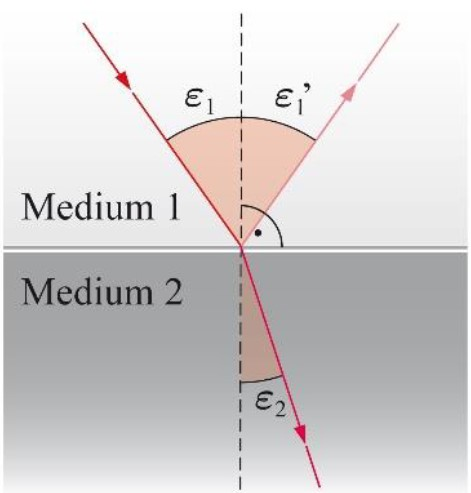
\includegraphics[width=\columnwidth, align=t]{images/brechung.jpg}
\end{minipage}
\hfill
\begin{minipage}[t]{0.64\columnwidth}
    $$ \boxed{ \frac{\sin(\varepsilon_1)}{\sin(\varepsilon_2)} = \frac{n_2}{n_1}  } \qquad \qquad
    \boxed{ v_i = \frac{c}{n_i}  } $$

    Je grösser $n$, desto grösser die Ablenkung und desto\\
    kleiner $\varepsilon$

    \medskip

    \begin{tabular}{@{}c l c@{}}
        $\varepsilon_i$ & Winkel zur Normalen & $[\varepsilon_i] = \degree$ \\
        $n_i$ & Brechungsindex & $[n_i] = 1$ \\
        $v_i$ & Geschwindigkeit im Medium $n_i$ & $[v_i] = \frac{\meter}{\second}$ \\
        $c$ & Lichtgeschwindigkeit $c = 300 \cdot 10^6 \, \frac{\meter}{\second}$ & $[c] = \frac{\meter}{\second}$
    \end{tabular}
\end{minipage}


\medskip

\paragraph{Anwendung: Glasfaser}

Der Lichtstrahl bliebt in der Kernzone (Medium 1) gefangen, da diese einen grösseren Brechungsindex hat als die Mantelschicht (Medium 2)
\begin{center}
    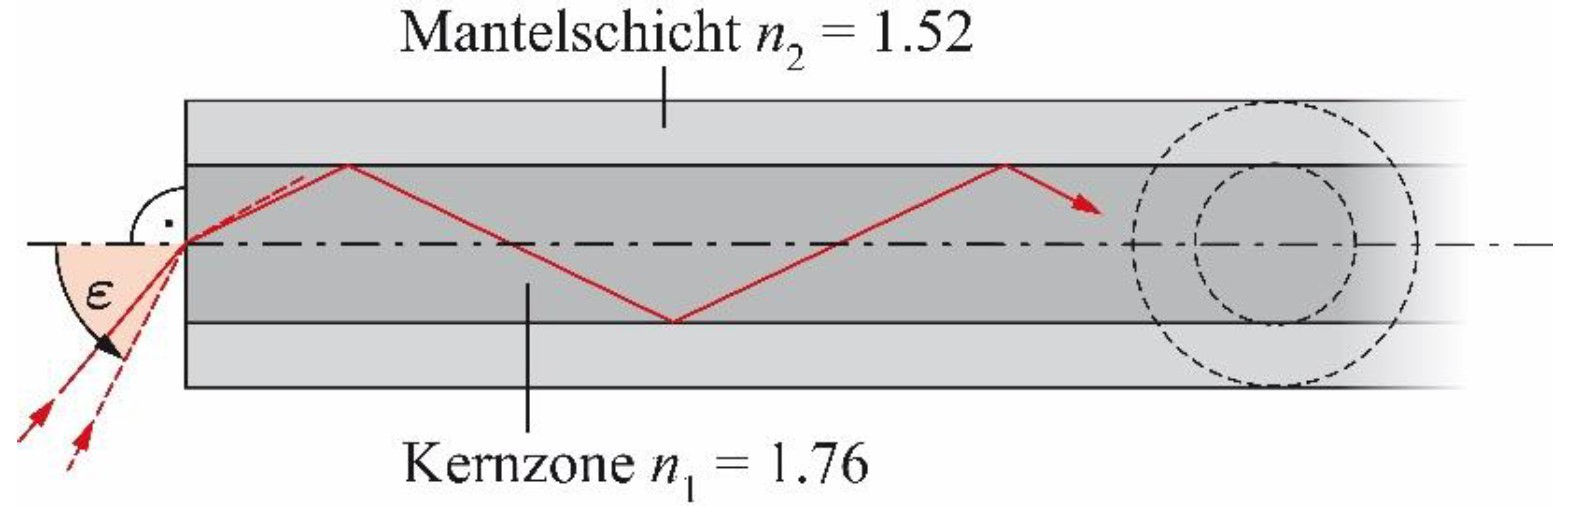
\includegraphics[width=0.75\columnwidth]{images/glasfaser.jpg}
\end{center}



\subsection{Totalreflexion}

\begin{minipage}[c]{0.6\columnwidth}
    Der Einfallswinkel $\varepsilon_1$ kann nicht grösser als 90° sein. \\
    Für $\varepsilon_1 = 90$° berechnet sich $\varepsilon_2 = \varepsilon_g$ aus: 
\end{minipage}
\hfill
\begin{minipage}[c]{0.38\columnwidth}
    $$ \varepsilon_g = \arcsin \left( \frac{n_1}{n_2} \right) $$
\end{minipage}

\smallskip

Für den Grenzfall von $\varepsilon_1 > 90$° wird der gesamte Stahl reflektiert.

\begin{center}
    \begin{minipage}{0.4\columnwidth}
        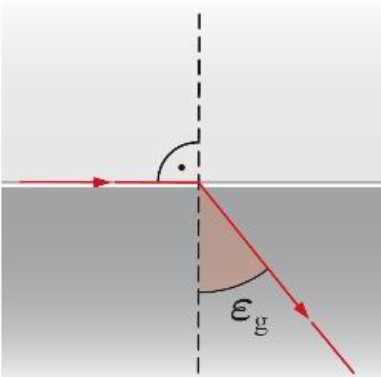
\includegraphics[height=3.5cm]{images/totalreflexion.jpg}
    \end{minipage}
    \begin{minipage}{0.4\columnwidth}
        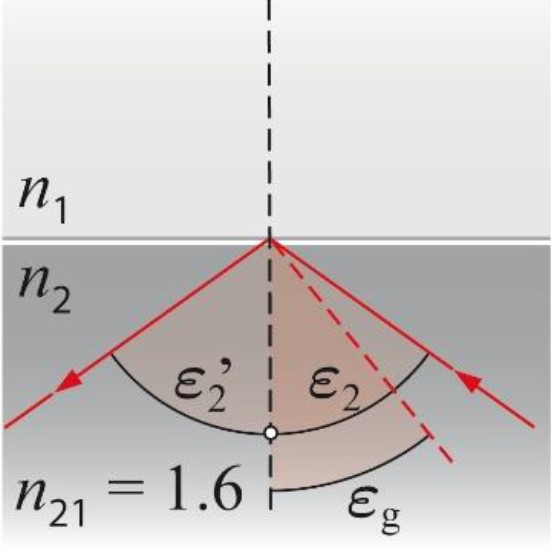
\includegraphics[height=3.5cm]{images/totalreflexion_2.jpg}
    \end{minipage}
\end{center}



\subsection{Brechung an ebenen Grenzflächen}

Ein Lichtstrahl wird verschoben bzw. in eine beliebige Richtung geändert

\begin{minipage}{0.32\columnwidth}
    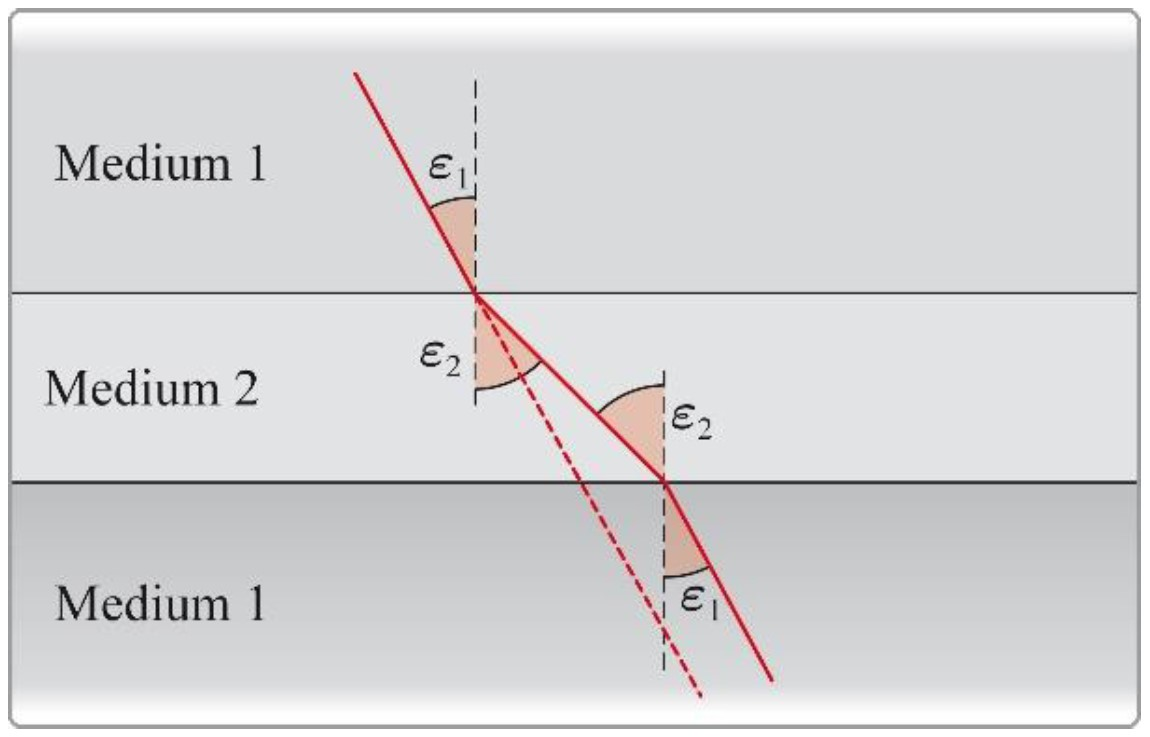
\includegraphics[width=\columnwidth]{images/verschiebung_lichtstrahl.jpg}
\end{minipage}
\hfill
\begin{minipage}{0.35\columnwidth}
    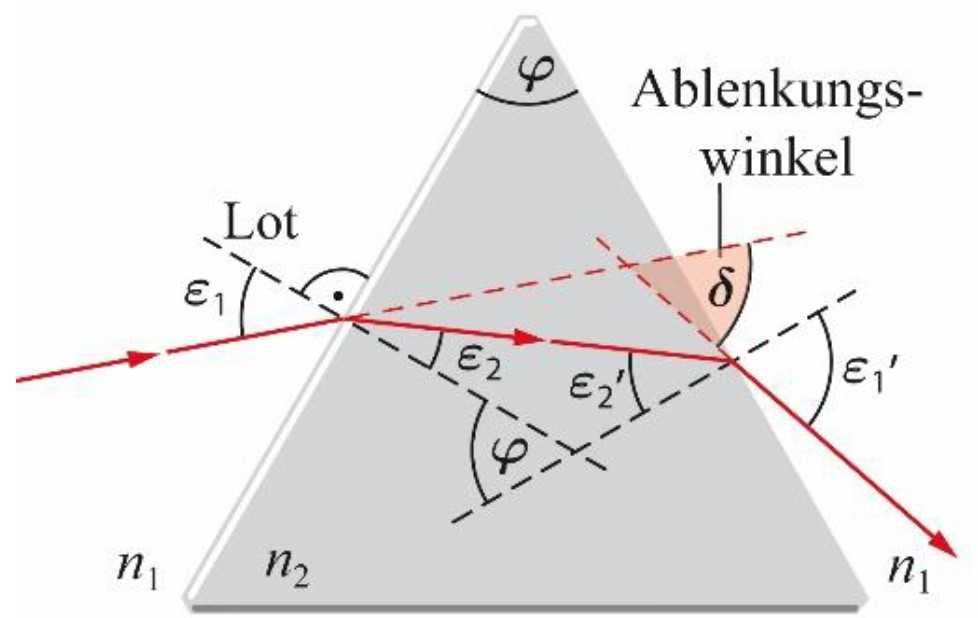
\includegraphics[width=\columnwidth]{images/prisma.jpg}
\end{minipage}
\hfill
\begin{minipage}{0.3\columnwidth}
    $$\boxed{ n = \frac{\sin (\varepsilon_1)}{\sin(\varepsilon_2)} = \frac{\sin \left(\frac{\varphi + \delta}{2} \right)}{\sin \left( \frac{\varphi}{2} \right)} } $$
\end{minipage}


\subsection{Brechung an gekrümmten Flächen}

Die Anwendung der Brechung ist eine Linse.

\medskip

\paragraph{Linsentypen}

\begin{minipage}{0.3\columnwidth}
    \centering
    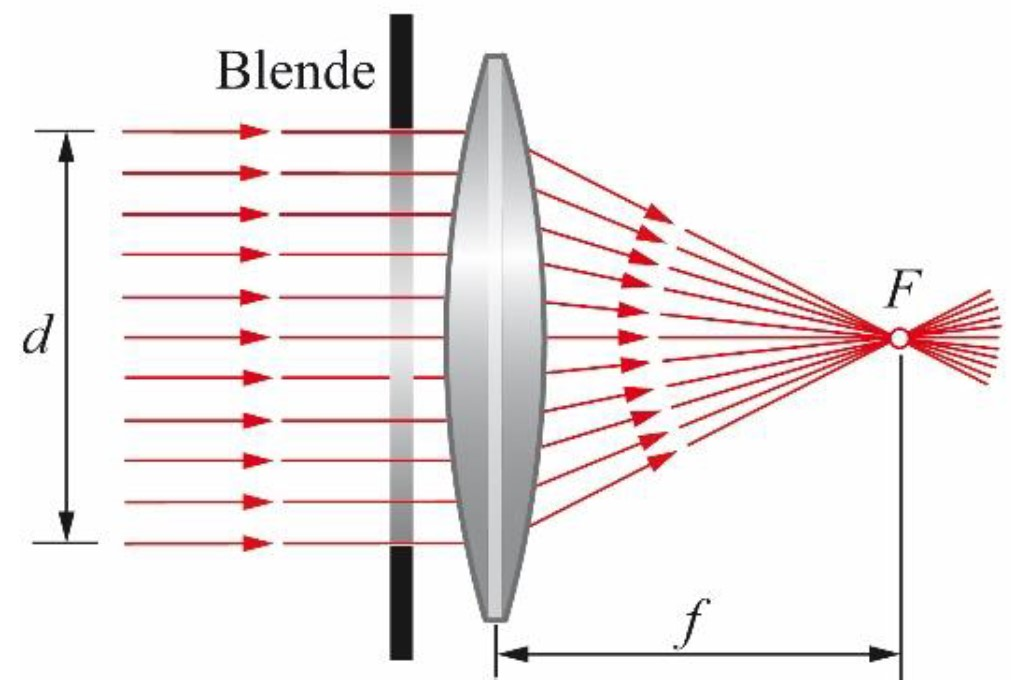
\includegraphics[height=2.0cm]{images/sammellinse.jpg}\\
    Sammellinse
\end{minipage}\hfill
\begin{minipage}{0.3\columnwidth}
    \centering
    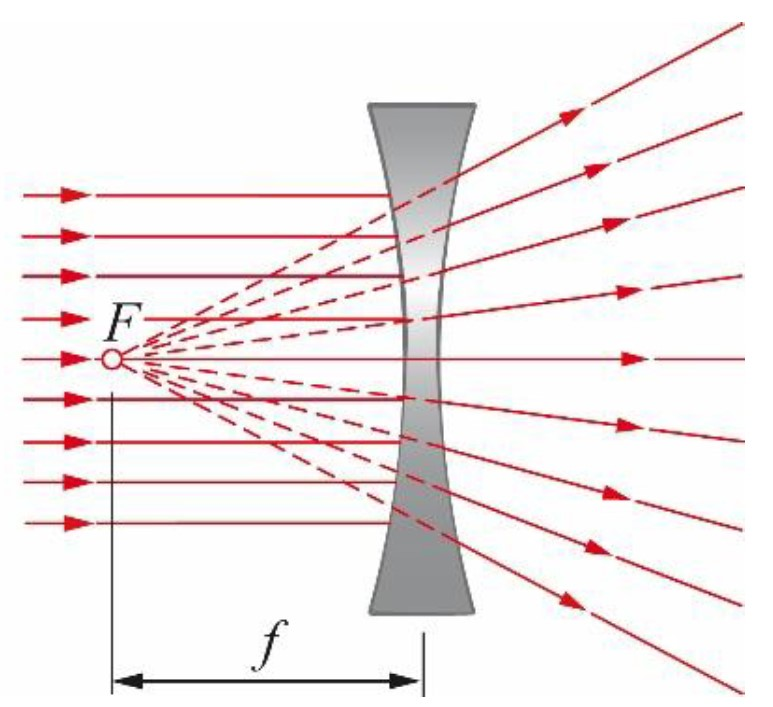
\includegraphics[height=2.0cm]{images/zerstreuungslinse.jpg}\\
    Zerstreuungslinse
\end{minipage}\hfill
\begin{minipage}{0.3\columnwidth}
    \centering
    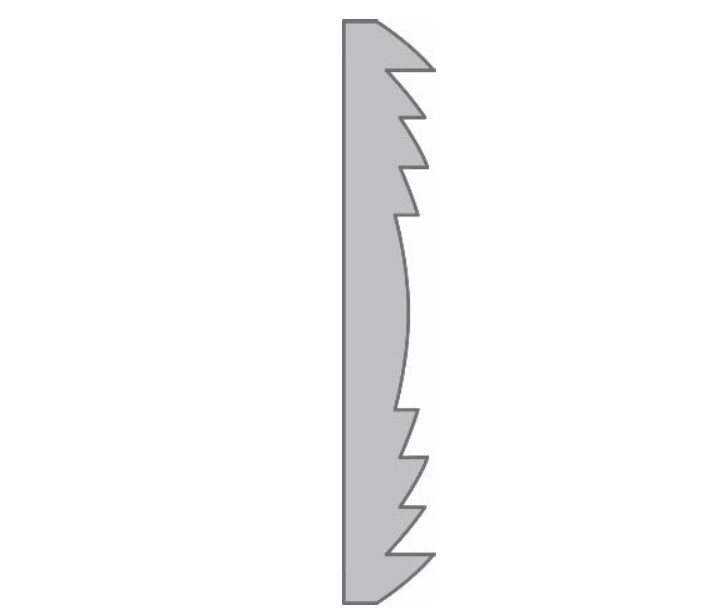
\includegraphics[height=2.0cm]{images/fresnellinse}\\
    Fresnellinse
\end{minipage}

\medskip
\textbf{Fresnellinse:} Es kann vermieden werden, dass die Linse eine übermässige Dicke aufweist. 


\example{Brechung mit  zwei Linsen}

\begin{center}
    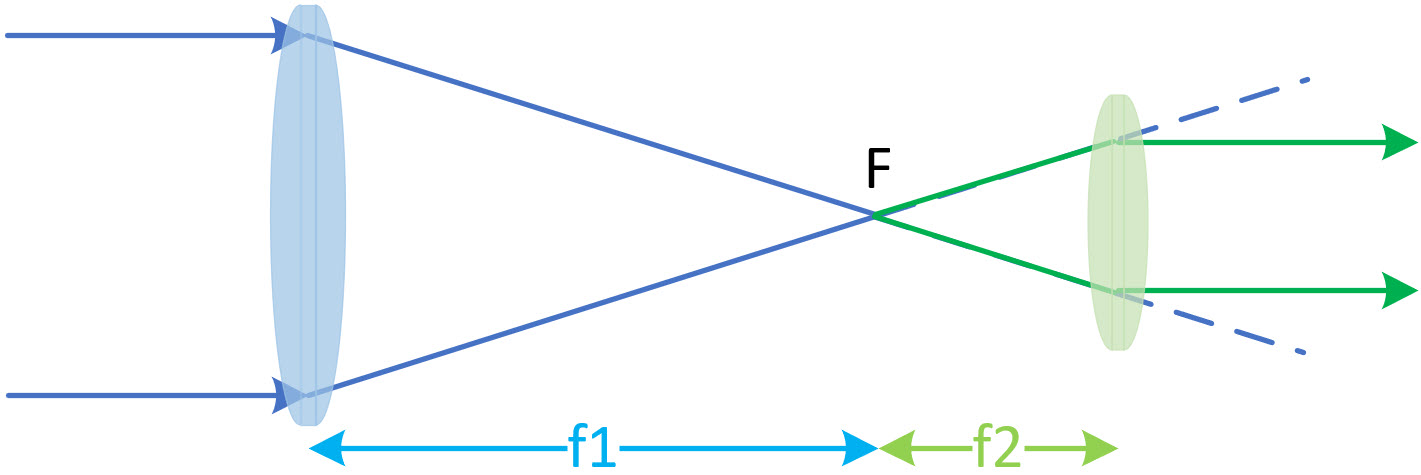
\includegraphics[width=0.85\columnwidth]{images/linsen.jpg}
\end{center}
Rechts gibt es ein kleineres Bild als links.


\subsection{Dispersion}\label{Dispersion Optik}

Der \textbf{Brechungsindex} eines Mediums ist eine \textbf{Funktion der Wellenlänge:} $n = n(\lambda)$ \\
Diese Wellenlängenabhängigkeit wird als \textbf{Dispersion} bezeichnet.
\[
    \boxed{ n^2(\lambda) = 1 + \frac{A}{ \frac{1}{\lambda_0^2} -  \frac{1}{\lambda^2} } }   \qquad \qquad
    \boxed{ n^2(f) = 1 + \frac{A'}{f_0^2 - f^2} }
\]


\subsubsection{Abbe Zahl $\bm{V}$}

Gibt an, wie stark dispersiv ein Material ist \\
Grosse Abbe-Zahl \textrightarrow\ wenig dispersives Material
